% Options for packages loaded elsewhere
\PassOptionsToPackage{unicode}{hyperref}
\PassOptionsToPackage{hyphens}{url}
%
\documentclass[
  a4paper]{article}
\usepackage{amsmath,amssymb}
\usepackage{lmodern}
\usepackage{iftex}
\ifPDFTeX
  \usepackage[T1]{fontenc}
  \usepackage[utf8]{inputenc}
  \usepackage{textcomp} % provide euro and other symbols
\else % if luatex or xetex
  \usepackage{unicode-math}
  \defaultfontfeatures{Scale=MatchLowercase}
  \defaultfontfeatures[\rmfamily]{Ligatures=TeX,Scale=1}
\fi
% Use upquote if available, for straight quotes in verbatim environments
\IfFileExists{upquote.sty}{\usepackage{upquote}}{}
\IfFileExists{microtype.sty}{% use microtype if available
  \usepackage[]{microtype}
  \UseMicrotypeSet[protrusion]{basicmath} % disable protrusion for tt fonts
}{}
\makeatletter
\@ifundefined{KOMAClassName}{% if non-KOMA class
  \IfFileExists{parskip.sty}{%
    \usepackage{parskip}
  }{% else
    \setlength{\parindent}{0pt}
    \setlength{\parskip}{6pt plus 2pt minus 1pt}}
}{% if KOMA class
  \KOMAoptions{parskip=half}}
\makeatother
\usepackage{xcolor}
\IfFileExists{xurl.sty}{\usepackage{xurl}}{} % add URL line breaks if available
\IfFileExists{bookmark.sty}{\usepackage{bookmark}}{\usepackage{hyperref}}
\hypersetup{
  pdftitle={Como a óptica influenciou a ciência: o telescópio},
  pdfauthor={Luiz Antônio Rangel},
  hidelinks,
  pdfcreator={LaTeX via pandoc}}
\urlstyle{same} % disable monospaced font for URLs
\usepackage[left=3cm,right=3cm,top=2cm,bottom=2cm]{geometry}
\usepackage{graphicx}
\makeatletter
\def\maxwidth{\ifdim\Gin@nat@width>\linewidth\linewidth\else\Gin@nat@width\fi}
\def\maxheight{\ifdim\Gin@nat@height>\textheight\textheight\else\Gin@nat@height\fi}
\makeatother
% Scale images if necessary, so that they will not overflow the page
% margins by default, and it is still possible to overwrite the defaults
% using explicit options in \includegraphics[width, height, ...]{}
\setkeys{Gin}{width=\maxwidth,height=\maxheight,keepaspectratio}
% Set default figure placement to htbp
\makeatletter
\def\fps@figure{htbp}
\makeatother
\setlength{\emergencystretch}{3em} % prevent overfull lines
\providecommand{\tightlist}{%
  \setlength{\itemsep}{0pt}\setlength{\parskip}{0pt}}
\setcounter{secnumdepth}{-\maxdimen} % remove section numbering
\usepackage{graphics} \usepackage[utf8]{inputenc} \usepackage[font=bf]{caption}

\fontsize{12}{22}
\ifLuaTeX
  \usepackage{selnolig}  % disable illegal ligatures
\fi

\title{Como a óptica influenciou a ciência: o telescópio}
\author{Luiz Antônio Rangel}
\date{}

\begin{document}
\maketitle

\hypertarget{introduuxe7uxe3o}{%
\section{1.0. Introdução}\label{introduuxe7uxe3o}}

Esse trabalho busca aprofundar no estudo da óptica a fim de mostrar, com
base na história, como a mesma influenciou diretamente na ciência e na
tecnologia, usando o telescópio como caso de estudo.

\hypertarget{introduzindo-a-uxf3ptica}{%
\section{1.1. Introduzindo a óptica}\label{introduzindo-a-uxf3ptica}}

Irei aqui introduzir brevemente o conteúdo de óptica, para entendimento
prévio de conceitos básicos que serão introduzidos posteriormente. A
óptica é considerada um gigantesco avanço para a humanidade pois, com
exceção de nossos olhos e memória, foi totalmente descoberta e depois
teve ferramentas baseadas em tal inventadas por nós.

\begin{figure}[!h]
\centering
    \caption{Equipe da CNN em Darã, na Arábia Saudita, durante a Guerra
do Golfo registrando imagens com uma filmadora profissional Sony SP BVP-50:}
    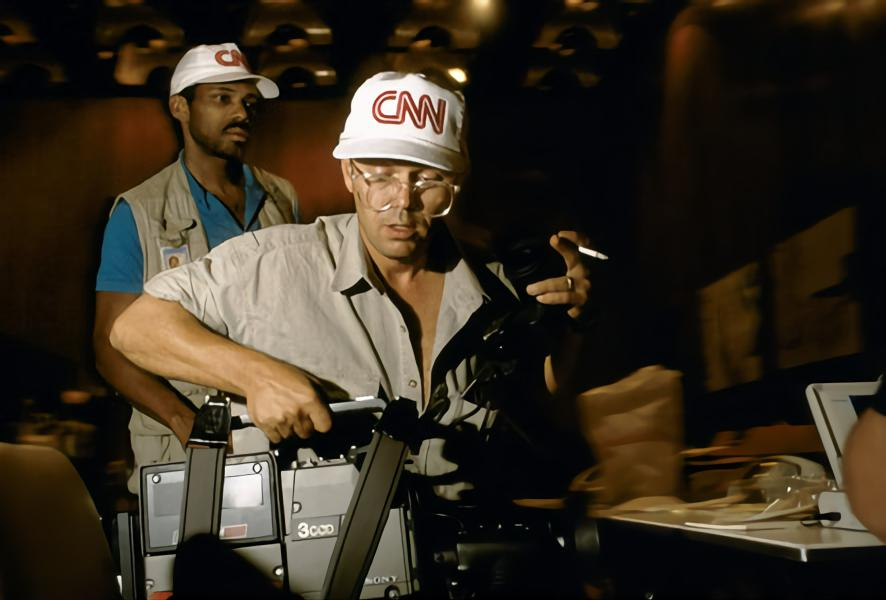
\includegraphics[]{../_img/61881601c180a.jpg}
Fonte: alamy.com  
\end{figure}

\newpage

A memória (fotográfica) artificial no caso é outra história diferente,
pois seria introduzida posteriormente (e rudimentarmente) pela primeira
vez em 1802, pelo químico britânico Thomas Wedgwood e seu colega Humphry
Davy em um informe chamado \emph{``An Account of a method of copying
Paintings upon Glass, and of making Profiles, by the Agency of Light
upon Nitrate of Silver''}, onde os dois descrevem o processo de se
``gravar'' silhuetas e sombras em superfícies cobertas com uma solução
de nitrato de prata dissolvido em água (proporção \(\frac{1}{10}\)).\\
75 anos antes, em 1727, o professor alemão Johann Heinrich Schulze já
havia conseguido ``gravar'' algumas palavras, mas usando uma solução
diferente da de Wedgwood e Humphry, sendo esta baseada em giz, nitrato
de prata e ácido nítrico.\\
Digo ``gravar'' entre aspas pois, em ambos os casos citados (e como
descrito no informe de Davy), a imagem iria descolorir em alguns
momentos caso não fosse mantida em um ambiente completamente sem luz.

\begin{quote}
``The copy of a painting, or the profile immediately after being taken,
must be kept in an obscure place. It may indeed be examined in the
shade, but in this case the exposure should be only for a few minutes;
by the light of candles or lamps, as commonly employed, it is not
commonly affected.\\
No attempts that have been made to prevent the uncoloured parts of the
copy, or profile, from being acted upon by light, have as yet been
successful.'' (DAVY, HUMPHRY, 1802; Pg. 242)
\end{quote}

\begin{figure}[!h]
\centering
    \caption{Imagem criada no século XIX a partir do processo descrito no informe de Davy:} 
    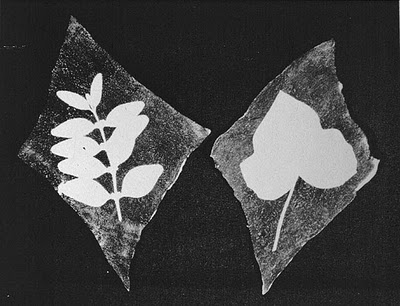
\includegraphics[width=100mm]{../_img/Facsimile-print_Thomas_Wedgwood.jpg}
    \linebreak
    Fonte: Wikimedia Commons, \textit{upado} em 9 de maio de 2010  
\end{figure}

\newpage

\hypertarget{o-que-uxe9-a-uxf3ptica}{%
\subsection{1.1.0. O que é a óptica?}\label{o-que-uxe9-a-uxf3ptica}}

A óptica é um dos seis ramos da física que estuda fenômenos envolvendo a
luz e a visão. Em contraste a alguns outros ramos das ciências exatas,
onde o conteúdo não é exatamente visível, a óptica é literalmente o que
se diz ao estudo do mundo visível. Alguns conceitos podem ser entendidos
com o auxílio de um laser, para se ter uma ideia.

Um breve fato curioso sobre a óptica, citado no começo do primeiro
capítulo de \emph{``Óptica Moderna: Fundamentos e Aplicações''} do Drº
Sérgio Carlos Zillo, é que há uma analogia entre ela e a mecânica
quântica; em que, no estado estacionário, ambas seriam descritas pela
mesma equação de ondas, além de alguns princípios/teoremas, como o
princípio da incerteza de Heisenberg, poderem ser provados usando
experimentos ópticos --- no caso do princípio da incerteza de
Heisenberg, seria possível prová-lo a partir de um experimento
envolvendo a difração da luz --- ou seja, o entendimento da mecânica
quântica se torna mais simples e menos abstrato se entendermos a óptica
antes.\\
Essa obra do Drº Zillo é, de fato, muito interessante; posteriormente
pretendo tirar algum tempo para lê-la.

\hypertarget{o-que-uxe9-a-luz}{%
\subsection{1.1.1. O que é a luz?}\label{o-que-uxe9-a-luz}}

\begin{quote}
``E disse Deus: Haja luz; e houve luz.''\\
- Gênesis 1:3
\end{quote}

Historicamente, a definição de luz já foi teorizada diversas vezes por
filósofos desde o século V a.C.; começando por Empédocles que, baseado
na sua crença de que tudo no Universo seria feito a partir de quatro
elementos, acreditava na ideia de que a deusa Afrodite havia criado o
olho humano a partir dos tais quatro elementos e que então havia
acendido uma chama que faria da visão algo possível ao permitir que o
olho fosse uma fonte de luz --- o que caiu por terra, pois se isso fosse
verdade, então o olho humano poderia capturar imagens tanto de dia
quanto à noite; ao pensar nisso, Epédocles propôs uma interação --- como
se fossem retas se ligando --- entre os raios de luz emitidos pelos
olhos e os raios de luz emitidos por outra fonte, como o próprio Sol,
por exemplo.\\
Em 300 a.C, Euclides escreveu \emph{``Optica''}, obra onde estudou a
luz, documentou e estudou matematicamente suas propriedades --- em que
questiona se o fenômeno da visão realmente seria resultado da interação
de raios proposta anteriormente por Empédocles, ao apontar o fato de
conseguir ver as estrelas imediatamente após piscar os olhos --- ou
seja, interrompendo o raio que sairia de seu olho e faria a interação,
sem nenhum tipo de ``\emph{delay}'' (como normalmente se esperaria de um
objeto em movimento, ou de uma perturbação mecânica no ambiente como o
próprio som) --- a partir desse questionamento, Euclides formulou duas
ideias: ou os raios emitidos pelo olho teriam velocidade positiva
infinita ou a hipótese de Empédocles estava simplesmente equivocada.

Em 55 a.C., Lucrécio escreveu em \emph{``De rerum natura''} que a ``luz
seria compostas de mínusculos átomos que, quando''empurrados'', não
perdem tempo em se disparar através do espaço na direção de seu
``empurrão''``.\\
Infelizmente não sei ler latim e nem grego, então vou ficar devendo o
trecho exato da obra.\\
Essa teoria foi percursora da ideia de fótons, que iria ser proposta e
reforçada por vários filósofos e cientistas, até ser derrubada pela
teoria de ondas em 1678, 1733 anos depois, formulada e publicada
inicialmente pelo polímata Christiaan Huygens em seu informe
\emph{``Traité de la lumière''} --- como não falo francês, também
ficarei devendo os trechos exatos em que Huygens faz e sustenta essa
ideia, \emph{excusez-moi} --- e posteriormente sustentada pelo
experimento do físico britânico Thomas Young, apresentado em seu informe
\emph{``On the theory of light and colours''} em que a luz apresentaria
características ondulatórias como a difração e também seria uma onda
transversal.

Nesta obra, ele também propõe que a visão seria composta principalmente
de três cores, que seriam ``canais nervosos'' nos olhos --- o que
futuramente iria ser, ao lado do triângulo de cores de Maxwell, base
para o padrão RGB, que é amplamente usado na eletrônica ---
principalmente na informática --- nos dias atuais.

\begin{quote}
``Since, for the reason here assigned by Newton, it is probable that the
motion of the retina is rather of a vibratory than of an undulatory
nature, the frequency of the vibrations must be dependent on the
constitution of this substance. Now, as it is almost impossible to
conceive each sensitive point of the retina to contain an infinite
number of particles, each capable of vibrating in perfect unison with
every possible undulation, it becomes necessary to suppose the number
limited, for instance to the three principal colours, red, yellow, and
blue, of which the undulations are related in magnitude nearly as the
numbers 8, 7, and 6; and that each of the particles is capable of being
put in motion less or more forcibly, by undulations differing less or
more from a perfect unison; {[}\ldots{]}'' (YOUNG, THOMAS, 1801, Pg. 19,
20)
\end{quote}

Young também fala sobre a opinião de Newton sobre o calor, em que
consistiria em vibração de partículas de um corpo, dizendo que foi
negada com pouca base e que possivelmente iria ter sua popularidade
recuperada:

\begin{quote}
``It was long an established opinion, that heat consists in vibrations
of the particles of bodies, and is capable of being transmitted by
undulations through an apparent vacuum. (Newt. Opt. Qu. 18.) This
opinion has been of late very much abandoned. Count Rumford, Professor
Pictet, and Mr.~Davy, are almost the only authors who have appeared to
favour it; but it seems to have been rejected without any good grounds,
and will probably very soon recover its popularity.'' (YOUNG, THOMAS,
1801, Pg. 32)
\end{quote}

E, ``encurtando'' todo o caminho matemático, histórico e teórico
percorrido por Young em seu informe, cá está a conclusão de que a luz é
uma onda --- ou, como ele chama, ondulações.

\begin{quote}
``This proposition is the general conclusion from all the pre­ ceding;
and it is conceived that they conspire to prove it in as satisfactory a
manner as can possibly be expected from the nature of the subject. It is
clearly granted by Newton, that there are undulations, yet he denies
that they constitute light; but it is shown in the three first
Corollaries of the last Proposi­ tion, that all cases of the increase or
diminution of light are referable to an increase or diminution of such
undulations, and that all the affections to which the undulations would
be liable, are distinctly visible in the phenomena of light; it may
there­ fore be very logically inferred, that the undulations are
light.'' (YOUNG, THOMAS, 1801, Pg. 44, 45)
\end{quote}

\begin{figure}[!h]
\centering
    \caption{Esquema da experiência de Young:} 
    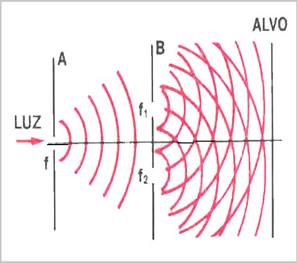
\includegraphics[width=60mm]{../_img/experiencia_de_young.jpg}
    \linebreak
    Fonte: Brasil Escola  
\end{figure}

A ideia de que a luz seria uma onda serviu de base para os estudos do
físico britânico James Clerk Maxwell, que mostraram que a luz seria uma
onda eletromagnética e que foram publicados em sua obra \emph{``A
Dynamical Theory of the Electromagnetic Field''}, ao lado de outras
descobertas extremamente importantes na área do eletromagnetismo, como a
das leis do eletromagnetismo.

\begin{quote}
``The agreement of the results seems to show that light and magnetism
are affections of the same substance, and that light is an
electromagnetic disturbance propagated through the field according to
electromagnetic laws.'' (MAXWELL, JAMES, 1865, Pg. 499)
\end{quote}

O informe de Maxwell teve um grande impacto, não só na área da óptica,
mas também na área do eletromagnetismo.\\
Diga-se de passagem, as ideias e descobertas de Maxwell foram um dos
pilares para a teoria quântica de Max Planck, na qual não vou me
aprofundar muito aqui pois já vai para uma parte bem mais avançada da
física; além dela rever e questionar vários conceitos já
pré-estabelecidos na Física Clássica, como a ideia de que uma onda nunca
transportará nada além de matéria.

Nessa explicação eu pulei muita história e várias teorias que surgiram
ao longo dos anos, a fim de pegar as teorias mais relevantes.

\hypertarget{um-pulinho-em-junho-redefinindo-o-conceito-de-ondas}{%
\subsection{1.1.2. ``Um pulinho em Junho'': redefinindo o conceito de
ondas}\label{um-pulinho-em-junho-redefinindo-o-conceito-de-ondas}}

\emph{Eu pensei que fosse interessante ``refrescar a memória'' no que se
diz ao conteúdo de ondas, sobre qual escrevi um ``mini-informe'' em
Junho de 2021, por conta do contexto deste trabalho --- admito que parte
também é ego, o que faz parte, para bem ou para o mal, de todo
acadêmico.}

\hypertarget{definiuxe7uxe3o}{%
\subsubsection{Definição}\label{definiuxe7uxe3o}}

A onda é a propagação de um movimento --- ou melhor dizendo, de sua
energia --- no ambiente com uma velocidade constante. Por ser apenas uma
propagação de energia, uma perturbação no ambiente, uma onda nunca
transportará nada, \textbf{absolutamente nada}, além de enegia.\\
Uma onda pode ser definida vetorialmente a partir das seguintes
variáveis:

\begin{itemize}
\tightlist
\item
  \(\gamma\) (Amplitude da onda, \(\mathbb{R}\));
\item
  \(\lambda\) (Comprimento de onda, \emph{m} ou
  \(\frac{\textit{cm}}{100}\));
\item
  \emph{t} (Período de tempo, \emph{s});
\item
  \emph{f} (Frequência de repetição, \emph{Hz})
\end{itemize}

\begin{figure}[!h]
\centering
    \caption{Vetor de uma onda:} 
    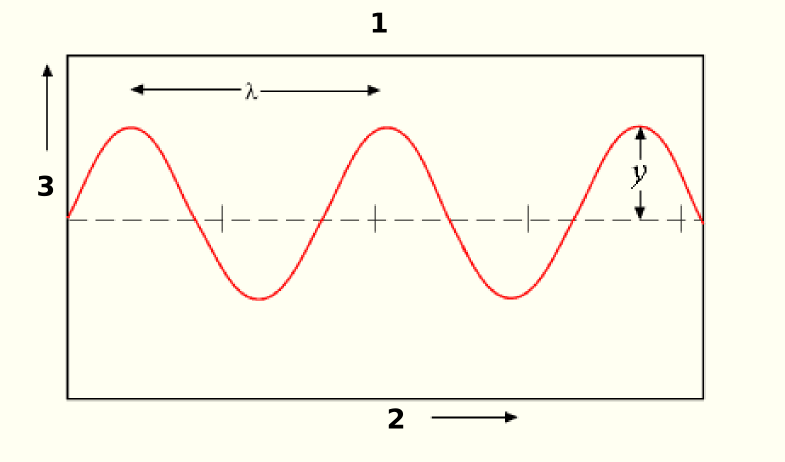
\includegraphics[width=100mm]{../_img/fig10.png}
    \linebreak
    Fonte: \textit{"Ondas: definição e demonstração"}, Rangel, Luiz Antônio \textit{et} Bertolucci, Antônio, 2021
\end{figure}

\hypertarget{meios-de-propagauxe7uxe3o}{%
\subsubsection{Meios de propagação}\label{meios-de-propagauxe7uxe3o}}

\begin{itemize}
\tightlist
\item
  Eletromagnético:

  \begin{itemize}
  \tightlist
  \item
    Resultado de um ``casamento'' entre um campo magnético e um campo
    elétrico; não dependem de um meio físico propriamente dito (eg.:
    ar).
  \end{itemize}
\item
  Mecânico:

  \begin{itemize}
  \tightlist
  \item
    Resultado de uma perturbação física (mecânica) no ambiente, logo,
    para haver perturbação mecânica, precisa-se de algum meio físico que
    possa ser perturbado (eg.: ar (de novo)).
  \end{itemize}
\end{itemize}

\hypertarget{direuxe7uxf5es-de-propagauxe7uxe3o}{%
\paragraph{Direções de
propagação}\label{direuxe7uxf5es-de-propagauxe7uxe3o}}

\begin{itemize}
\tightlist
\item
  Longitudinal:

  \begin{itemize}
  \tightlist
  \item
    Paralelo à perturbação. Ondas sonoras (mecânicas) se propagam
    paralelamente à sua perturbação.
  \end{itemize}
\item
  Transversal:

  \begin{itemize}
  \tightlist
  \item
    Perpendicular à perturbação. Ondas de choque (mecânicas) e ondas de
    luz (segundo Young) se propagam perpendicularmente à sua
    perturbação.
  \end{itemize}
\end{itemize}

\hypertarget{dimensuxf5es}{%
\subsubsection{Dimensões}\label{dimensuxf5es}}

\begin{itemize}
\tightlist
\item
  Unidimensionais;

  \begin{itemize}
  \tightlist
  \item
    A energia se propaga em uma única direção no ambiente, de forma
    linear.
  \end{itemize}
\item
  Bidimensionais;

  \begin{itemize}
  \tightlist
  \item
    A energia se propaga em duas direções, em um plano.
  \end{itemize}
\item
  Tridimensionais;

  \begin{itemize}
  \tightlist
  \item
    A energia se propaga em três direções, em um espaço tridimensional
    --- que, geralmente, é representado como uma esfera.
  \end{itemize}
\end{itemize}

\hypertarget{fenuxf4menos}{%
\subsubsection{Fenômenos}\label{fenuxf4menos}}

\begin{itemize}
\tightlist
\item
  Difração

  \begin{itemize}
  \tightlist
  \item
    A onda contorna um obstáculo, como uma parede por exemplo.\\
    Entretanto, como não existe almoço grátis, ela perde sua
    intensidade.
  \end{itemize}
\item
  Reflexão

  \begin{itemize}
  \tightlist
  \item
    A onda faz o movimento inverso, sem perder nenhuma propriedade,
    apenas invertendo sua direção.
  \end{itemize}
\item
  Refração

  \begin{itemize}
  \tightlist
  \item
    A velocidade da onda difere --- geralmente a causa para isso é a
    densidade do meio --- o que causa uma distorção.
  \end{itemize}
\item
  Ressonância

  \begin{itemize}
  \tightlist
  \item
    A onda entra em contato com um corpo em vibração igual ou
    semelhante, resultando na absorção da onda pelo dito corpo, o que
    consequentemente aumenta sua vibração interna.
  \end{itemize}
\end{itemize}

\hypertarget{o-telescuxf3pio}{%
\section{2.0. O telescópio}\label{o-telescuxf3pio}}

\hypertarget{o-que-uxe9}{%
\subsection{2.0.1. O que é?}\label{o-que-uxe9}}

O telescópio é um instrumento óptico criado com a finalidade de se
observar objetos distantes do observador com tamanho maior; geralmente é
usado dentro da astronomia, para a observação de astros.

\hypertarget{um-pouco-de-contexto-histuxf3rico}{%
\subsection{2.0.2. Um pouco de contexto
histórico}\label{um-pouco-de-contexto-histuxf3rico}}

O uso de prévio de lentes para ampliar corpos já era feito desde a época
da Grécia antiga, mas o primeiro registro de algo próximo de um
telescópio foi feito em 1608, a partir de uma patente feita por Hans
Lippershey, um fabricante de lentes dos Países Baixos, que consistia de
se usar duas lentes em série para aumentar objetos distantes. A ideia
originalmente não era dele, mas sim de um aprendiz que percebeu que,
quando colocava duas lentes em série, conseguia ver objetos distantes de
perto.

\begin{figure}[!h]
\centering
    \caption{Imagem descrevendo como o sistema de lentes em série funcionava:} 
    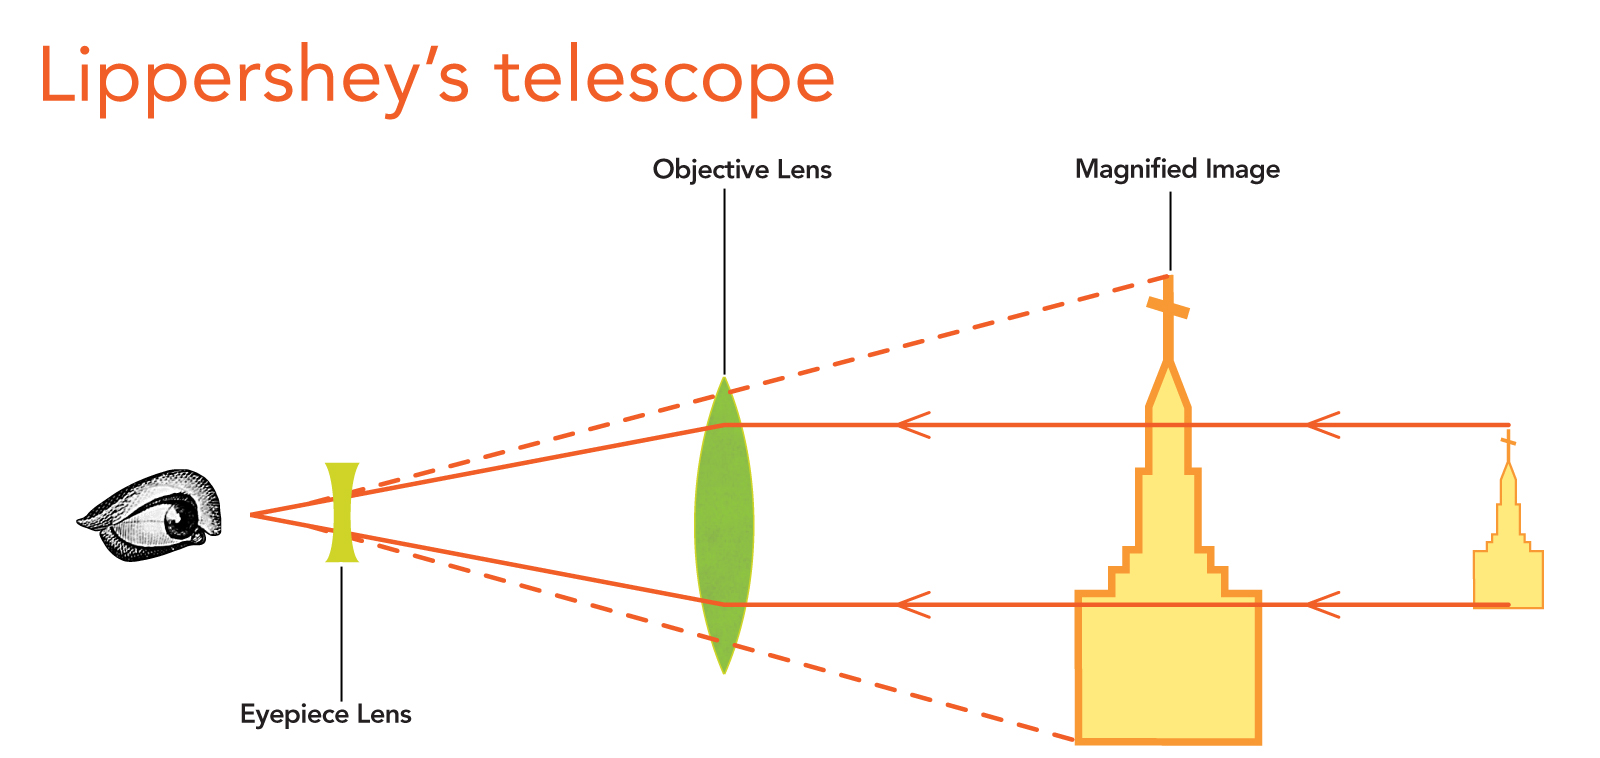
\includegraphics[width=100mm]{../_img/Untitled-1_1.jpg}
    \linebreak
    Fonte: Corning Museum of Glass 
\end{figure}

Por ser algo muito, digamos, direto de se fazer e resultado de um
verdadeiro simples posicionamento, Lippershey acabou não só por não ter
direito à patente como também foi acusado de plágio por seus
concorrentes locais, entre eles Zacharias Janssen, que afirmou, após a
publicação da ideia do telescópio como sendo de Lippershey, ter criado
uma ferramenta similar quatro anos antes, em 1604.

Inicialmente o telescópio não era pensado como uma ferramenta para o
estudo de astros, mas sim como uma ferramenta para se visualizar coisas
distantes --- inclusive, Lippershey teria vendido-os inicialmente para o
governo holandês, como uma ferramenta militar.

Um ano após a publicação do ``invento'' de Lippershey, em 1609, o físico
e astrônomo italiano Galileu Galilei decidiu fabricar seu próprio
telescópio, que no final acabou por ter uma funcionalidade superior ao
de Lippershey, podendo ampliar aproximadamente o triplo do que o modelo
de Lippershey em sua ``primeira versão''.

Com isso, ele conseguiu o respeito dos oficiais da cidade-Estado de
Veneza e dos acadêmicos da Universidade de Padua. Além disso, como já se
é conhecido, Galileu também estudou os astros e foi o primeiro a de fato
provar que o modelo geocêntrico estaria errado, o que levou à sua
perseguição pela Igreja Católica na época --- o que é, de certa forma,
decepcionante se lembrarmos que Galileu nunca negou a existência de
Deus, inclusive defendia que a ciência humana e Deus deveriam andar
juntos, afinal um seria a tentativa de entender a criação de outro.

\begin{figure}[!h]
\centering
    \caption{Ilustração de Galileu observando as luas de Júpiter e as fases
de Vênus:} 
    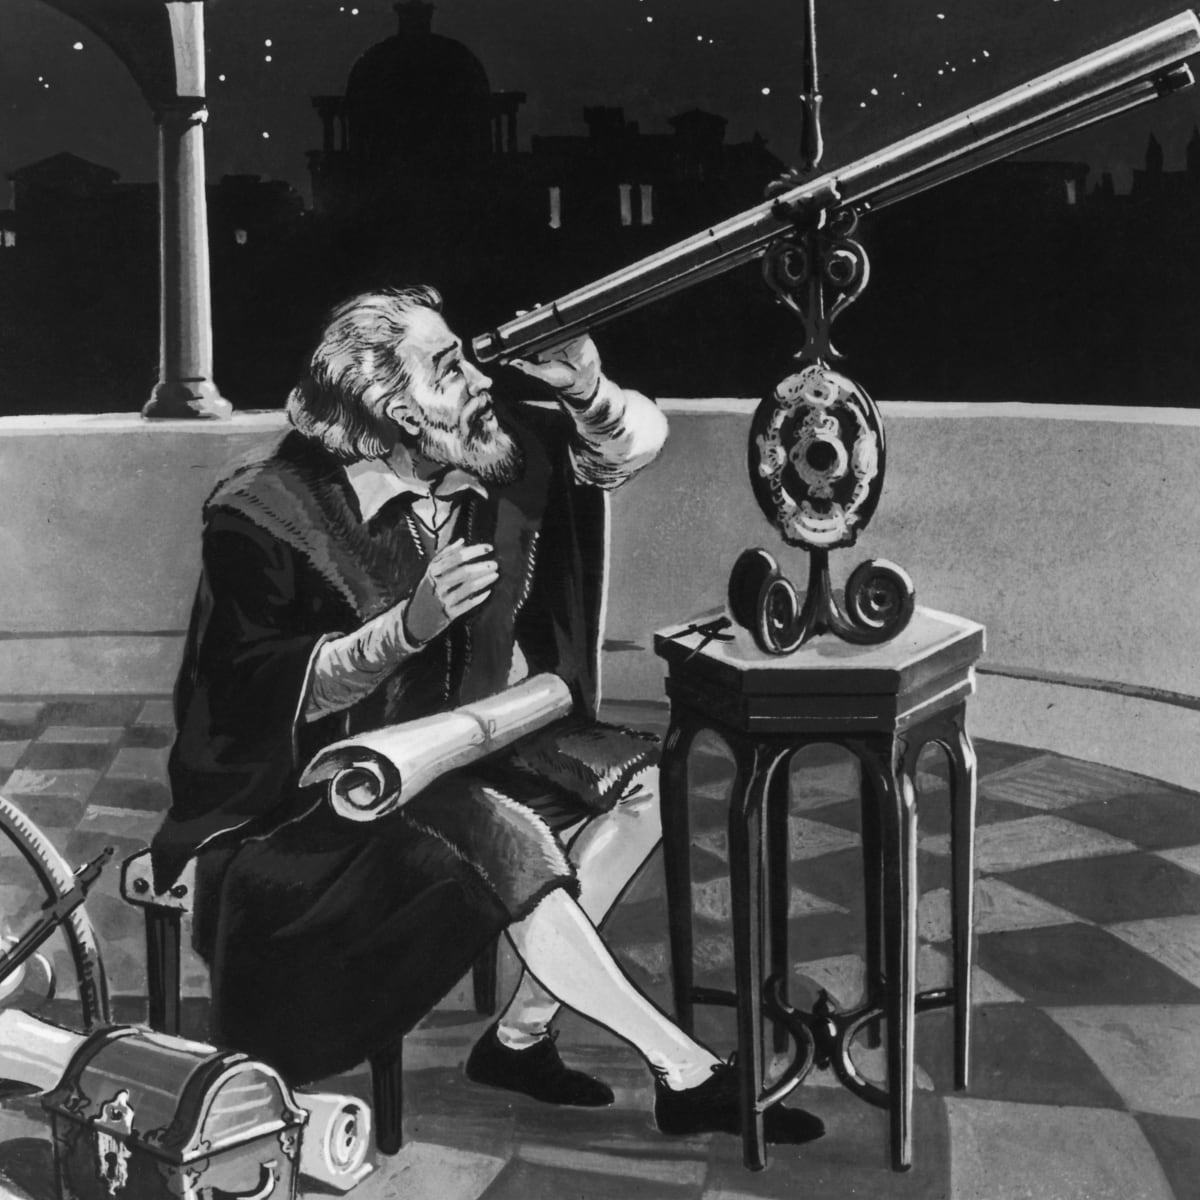
\includegraphics[width=100mm]{../_img/galileo-galilei-discovers-the-moons-of-jupiter-and-the-phase-of-venus.jpg}
    \linebreak
    Fonte: Desconhecida; possivelmente Domínio Público
\end{figure}

\newpage

Um ano após Galileu ter fabricado seu telescópio, em 1610, o matemático
alemão Johannes Kepler ganhou um telescópio e, mesmo não tendo aptidão
em engenharia (e estando com baixa visão) para montar um do zero, Kepler
sabia o que podia ser melhorado ou não. Rapidamente, várias melhoras
foram propostas por ele e aplicadas.\\
Kepler teve uma ideia de se montar um telescópio mais longo, com uma
lente ocular convexa junto com uma lente objetiva também convexa. A
ideia dele permitia que houvesse um maior campo de visão e ampliação do
que a ideia de Galileu original, a única desvantagem era o fato da
imagem estar de ponta-cabeça, mas se tratando do céu não era um
problema, afinal os planetas e satélites naturais são simétricos.

Os telescópios, todavia, ainda tinham diversos problemas que seriam
eventualmente corrigidos, um deles era a aberração cromática, onde a luz
sofre diferença de refração entre as lentes, ou seja, as cores se
dispersam.

\begin{figure}[!h]
\centering
    \caption{Aberração cromática:} 
    
\includegraphics[width=60mm]{../_img/Numero-ABBE-BLOG-2.png}
    \linebreak
    Fonte: Lentes Luxxor
\end{figure}

A solução para esse problema já era de certa forma conhecida: um
telescópio refletor, que usasse um espelho esférico para captar imagens
ao invés de uma série de lentes convexas. Tinha-se a ideia na mão, mas
ninguém tinha conseguido montar um telescópio desses que funcionasse até
então.\\
Em 1668, 58 anos depois do telescópio de Kepler, Newton havia coneguido
montar seu primeiro telescópio refletor com sucesso.\\
Teoricamente ele é simples, consiste de um espelho esférico côncavo que
capturava a luz e então refletia essa imagem num espelho plano que, por
último, refletia na lente ocular, mas montar na prática tende a ser
complexo.

\begin{figure}[!h]
\centering
    \caption{Diagrama do caminho da luz dentro de um telescópio Newtoniano:} 
    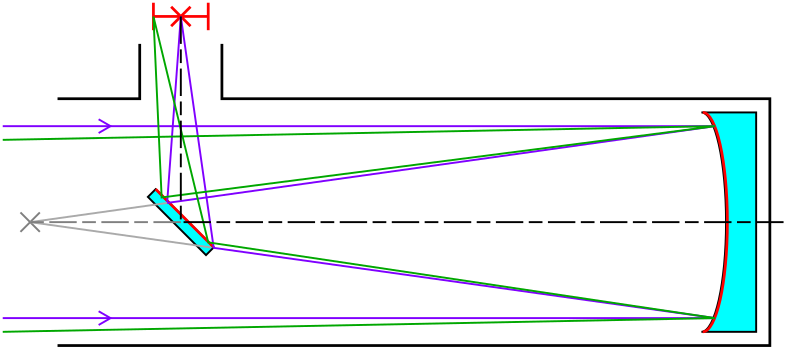
\includegraphics[width=60mm]{../_img/800px-Newtonian_telescope2.svg.png}
    \linebreak
    Fonte: Wikimedia Commons, trabalho original por Krishnavedala
\end{figure}

Assim como na história da luz, eu também acelerei bastante a linha do
tempo, a fim de contar apenas o que foi importante e deixar clara a
ideia principal do telescópio: é uma ferramenta feita utilizando-se um
conjunto (também chamado ``jogo'') de lentes ou espelhos, a fim de
ampliar um corpo distante.

\hypertarget{o-que-suxe3o-lentes}{%
\subsection{2.0.3. O que são lentes?}\label{o-que-suxe3o-lentes}}

\begin{figure}[!h]
\centering
    \caption{Keitaro Urashima olhando para o céu:} 
    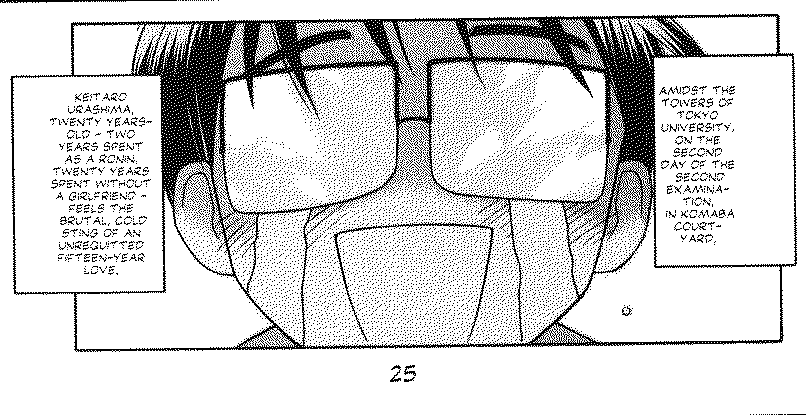
\includegraphics[width=100mm]{../_img/keitaro_urashima_glasses.png}
    \linebreak
    Fonte: Love Hina, Vol. III HINATA 016. \textit{"Birth of the Tokyo University Couple!"} 
\end{figure}

As lentes são peças que interagem com a luz --- chamadas formalmente de
sistemas ópticos --- utilizadas para produzir desvios nos raios de luz
que incidem sobre elas, se ``aproveitando'' da propriedade da refração
presente na luz, a fim de concentrá-los em um ponto específico --- como
em lentes de óculos, por exemplo.

Lentes que fazem os raios paralelos ao seu eixo central se aproximarem
dele ainda mais são chamadas ``lentes \emph{convergentes}'', pois
convergem os raios em um único ponto, já lentes que fazem com que esses
raios se afastem de seu eixo central são chamadas ``lentes
\emph{divergentes}'', pois divergem os raios para outro ponto. As
propriedades que realmente ditam como a luz deve ser refratada são a sua
geometria e seu índice de refração e, diga-se de passagem, o famigerado
``grau'' é a capacidade defletir os raios, chamada de diotropia.\\
As lentes dividem-se em duas classificações gerais: côncavas e convexas,
que são, respectivamentente, lentes de bordas grossas e bordas finas.

\begin{figure}[!h]
\centering
    \caption{Símbolo usado em diagramas para indicar qual é o tipo da lente:} 
    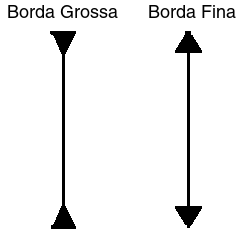
\includegraphics[width=50mm]{../_img/borda_grossa_e_fina_lentes.png}
    \linebreak
        Fonte: Imagem autoral
\end{figure}

Existem seis formatos/classificações de lentes, que são nomeadas a
partir de um observador externo, que observa suas faces, e que podem ser
\emph{côncavas} ou \emph{convexas}.

\begin{figure}[!h]
\centering
    \caption{Classificações de lentes:} 
    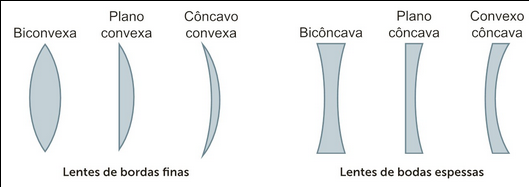
\includegraphics[width=70mm]{../_img/classificacoes_lentes_esfericas.png}
    \linebreak
        Fonte: CNEC Física - 2ª Série do Ensino Médio Vol. III 
\end{figure}

Cada classificação tem uma capacidade de desviar os raios de luz, essa
capacidade é explicada pela equação dos fabricantes de lentes (também
conhecida como ``equação de Halley'').

\begin{figure}[!h]
\centering
    \caption{Elementos geométricos de uma lente esférica:} 
    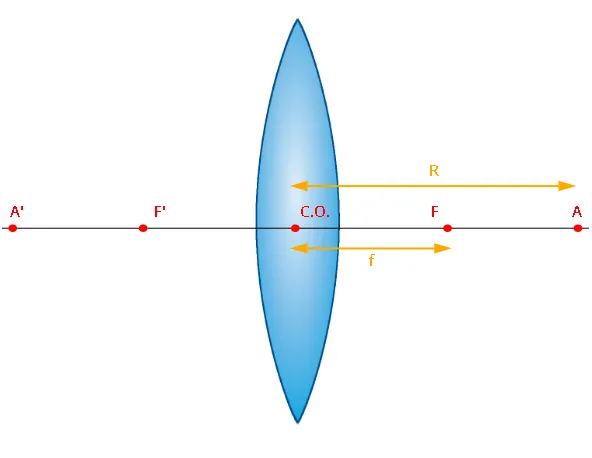
\includegraphics[width=70mm]{../_img/elementos-geometricos.png}
    \linebreak
        Fonte: Mundo Educação - UOL 
\end{figure}

Toda lente esférica, independente da classificação, têm essas variáveis
em comum:

\begin{itemize}
\tightlist
\item
  centro (\emph{O});
\item
  foco principal do objeto (\emph{F});
\item
  foco principal da imagem (\emph{F\^{}I});
\item
  foco antiprincipal do objeto (também conhecido como centro de
  curvatura em espelhos esféricos) (\emph{C});
\item
  foco antiprincipal do objeto (também conhecido como centro de
  curvatura em espelhos esféricos) (\emph{C\^{}I});
\end{itemize}

Essas variáveis são usadas para tudo que envolva algum tipo de cálculo
dentro desse assunto. Normalmente --- para não dizer ``sempre'' --- os
cálculos se baseiam em proporções ou razões.\\
Um exemplo é o cálculo de dioptria, que é feito usando uma razão de
\(\frac{1}{f}\), onde \emph{f} é a distância focal (distância entre o
centro \emph{O} e o foco principal do objeto \emph{F}):\\
\textbf{Nota}: É medido em \emph{di}, não é uma variável especial.\\
\scalebox{2}{ C = $\frac{1}{f}$ $\textit{di}$}

Outra fórmula usada é a fórmula da ampliação, que é uma razão de
\(\frac{i}{o}\), onde \emph{i} é o tamanho da imagem e \emph{o} é o
tamanho do objeto:\\
\scalebox{2}{ A = $\frac{i}{o}$ }

E, por último, temos a equação de Gauss, também chamada de equação dos
pontos conjugados, baseado nos raios notáveis, onde \emph{f} é a
distância focal, \(p^{o}\) é a posição do objeto e \(p^{i}\) é a posição
da imagem, normalmente em centímetros ou metros em relação ao centro
óptico:

\scalebox{2}{ $\frac{1}{f}$ = $\frac{1}{p^o}$ + $\frac{1}{p^i}$ }

\begin{figure}[!h]
\centering
    \caption{Raios notáveis:} 
    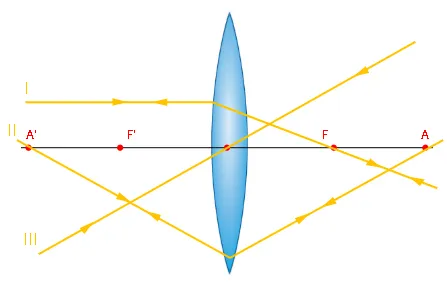
\includegraphics[width=70mm]{../_img/raios-notaveis.png}
    \linebreak
        Fonte: Mundo Educação - UOL 
\end{figure}

Algo que vale se lembrar (ou notar) é que essas fórmulas --- assim como
algumas regras --- são ``importadas'' dos espelhos esféricos.

\newpage

\hypertarget{o-cuxf4ncavo-e-o-convexo}{%
\subsection{2.0.4. O Côncavo e o
Convexo}\label{o-cuxf4ncavo-e-o-convexo}}

\begin{figure}[!h]
\centering
    \caption{Motoko Aoyama se observando num espelho:} 
    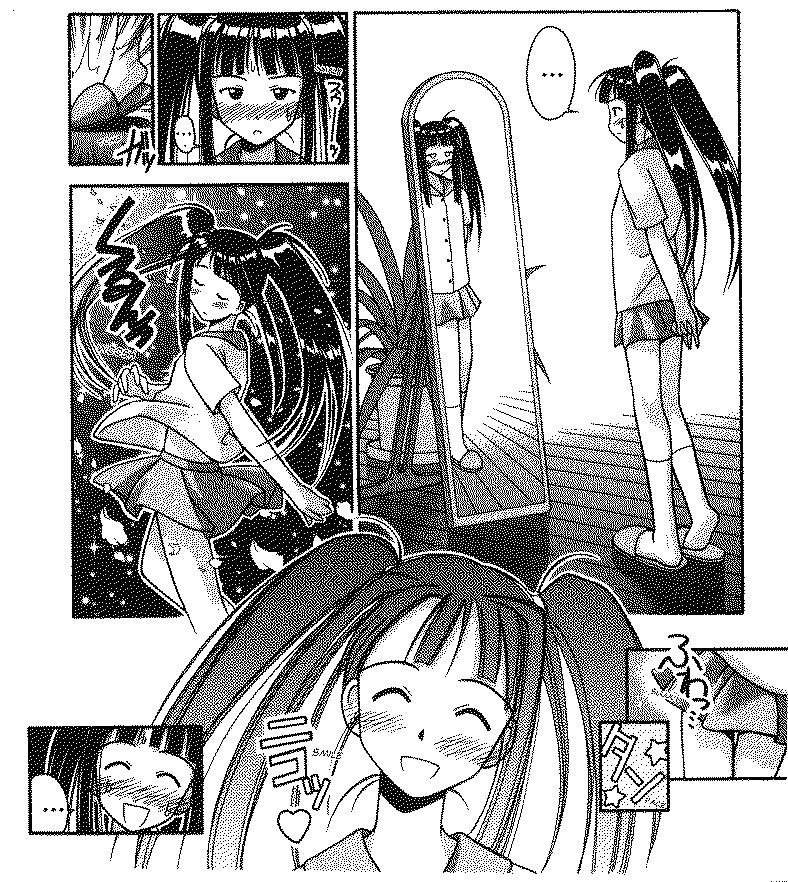
\includegraphics[width=70mm]{../_img/motoko_aoyama_convex_mirror.png}
    \linebreak
    Fonte: Love Hina, Vol. IV HINATA 027. \textit{"Kendo Girl's Tiny Little Problem"}  
\end{figure}

Nessa imagem, retirada do mangá \emph{``Love Hina''}, podemos ver uma
garota se observando num espelho de corpo \textbf{aparentemente} plano,
mas vemos que sua imagem aparece menor no espelho do que na prática ---
algo que não aconteceria caso o espelho fosse realmente plano --- ou
seja, esse espelho é esférico e podemos deduzir que tem um raio de
curvatura pequeno.

Mas o que esse espelho seria? Côncavo ou convexo?\\
Essa é uma dúvida que muitas vezes bate em você como um caminhão de
bombeiro bate numa motocicleta em uma autoestrada no meio de uma
avaliação.

\begin{quote}
``Espera, o foco é positivo ou negativo? Me disseram que o espelho é
côncavo no enunciado\ldots{}''
\end{quote}

\begin{figure}[!h]
\centering
    \caption{As "calotas" e suas superfícies:} 
    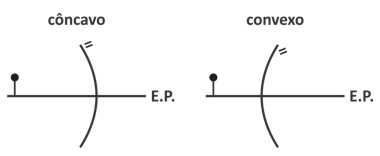
\includegraphics[width=70mm]{../_img/Screenshot_2921.jpg}
    \linebreak
    Fonte: Proenem 
\end{figure}

De fato, a garota está em frente a um espelho convexo, onde a camada que
reflete os raios de luz é externa à ``calota'', pois sua imagem está
sendo \textbf{diminuída}.\\
Em um espelho côncavo, onde a camada que reflete os raios de luz é
interna à ``calota'', sua imagem estaria sendo ampliada.

\newpage

\hypertarget{conclusuxe3o}{%
\section{3.0. Conclusão}\label{conclusuxe3o}}

Neste trabalho nós observamos e exploramos não só o contexto histórico
do telescópio, mas também da óptica no geral, além de reforçarmos
teoricamente conceitos importantes como os de espelhos esféricos.

\hypertarget{detalhes-tuxe9cnicos}{%
\subsubsection{3.0.1 Detalhes técnicos}\label{detalhes-tuxe9cnicos}}

Este trabalho foi feito usando o Pandoc, uma ferramenta de código-aberto
para UNIX e Microsoft Windows que permite escrever Markdown e LaTeX
simultaneamente; também foi feito com o uso de ferramentas de linha de
comando do UNIX, como \texttt{sed}, \texttt{grep}, \texttt{find}, o
editor de texto Vim e a suite ImageMagick.\\
Tudo que fora feito de forma autoral por mim, Luiz Antônio, está na
licença Creative Commons Attribution 4.0, análoga a domínio público, com
a exceção de créditos apenas.

\end{document}
